\documentclass[journal, 11pt]{IEEEtran}

\usepackage{epsfig,rotating,setspace,latexsym,amsmath,epsf,amssymb,bm,amsbsy}
\usepackage{cite,graphicx,color,subfigure,here}
\usepackage{amsmath}
\usepackage[normalem]{ulem} 
\usepackage{algorithm}
\usepackage[noend]{algpseudocode}
\usepackage{epstopdf}
\usepackage{scrextend}
\usepackage{ifpdf}
\usepackage{authblk}
\usepackage{caption2}
\usepackage{caption3}
\usepackage[english]{babel}
\usepackage{dsfont}

\newcommand{\ba}{\begin{align}}
\newcommand{\ea}{\end{align}}


\begin{document}
\title{Cognition in Connected Vehicles}

\author{Bengi Aygun$^\dag$, Mahni Shayganfar$^*$, and Alexander M. Wyglinski$^\dag$\\
\normalsize $^\dag$Department of Electrical and Computer Engineering, Worcester Polytechnic Institute, Worcester, MA\\
\normalsize $^*$Department of Computer Science, Worcester Polytechnic Institute, Worcester, MA\\
\normalsize Email: \{baygun, alexw\}@wpi.edu, mshayganfar@wpi.edu}

\maketitle

\begin{abstract}
In this paper,
\end{abstract}

\begin{keywords}
cognition, connected vehicles ...
\end{keywords}%

\IEEEpeerreviewmaketitle
\section{Introduction}
%
Intelligent transportation systems (ITS) will form an integral part of society's
transportation infrastructure within few years.

\subsection{Roads as Social Environments}

A social environment refers to an individual's physical surroundings, resources
and social relationships. A social relationship includes the interaction between
two or more individuals in the environment. A social relationship is the most
dynamic part of a social environment. Hence, developing and maintaining positive
social relationships is crucial for a social environment and is influenced by
the individuals' quality of interaction. Roads are social environments in which
individual vehicles interact with each other through their ``nonverbal"
behaviors obeying the same traffic law. However, there are many violations of
the laws on the roads all over the world in daily basis which consequently leads
to expensive and sorrowful failures. What causes these failures is mostly the
failure of the drivers to effectively interpret their driving environment and
make an appropriate decision with respect to their constraints such as lack of
time, lack of perception, and plethora of cognitive load. Therefore, it is
crucial to involve awareness in the vehicles to share the meaning of what they
dynamically perceive rather than broadcasting the data coming from their sensory
system. For example, any sensory information leading to an alert on a particular
vehicle does not necessarily have the same meaning both for the occupants and
the neighbors of that vehicle. The alert warns the occupants of the vehicle to
be aware of an internal failure (e.g., malfunction in the transmission system),
or an external adversary (e.g., an unexpected leaping of an animal into the
road). The same alert has a different meaning for the close vehicle approaching
from behind; no matter what caused the alert in the leading vehicle, the
posterior vehicle should slow down effective immidiately. However, the same
alert can be interpreted in a totally different way for a neighbor in front of
the originally alerted vehicle. In fact, this vehicle can ignore the received
alert and continue the safe drive. Ultimately, these type of improvements leads
to a higher quality of vehicles' interaction which consequently increases the
safety of the roads.

\subsection{Driving Needs Pareto Optimal Decisions}

Cognitive architectures are used to solve high-dimensional multi-objective
tasks and to make proper decisions with respect to the dynamics of such
environments. Most of the time the real world problems possess a high level of
complexity due to the dynamism involved in the environment. A social environment
is an example of such complex environments. A social environment includes humans
as variety of sources making decisions independently but interrelated to each
other. Roads are social environments and driving is the social act of drivers'
behavior. It is clear that driving involves many decisions in which a driver
needs to maintain its own objectives while recognizing objectives of the others.

\begin{figure}[tbh]
  \centering
  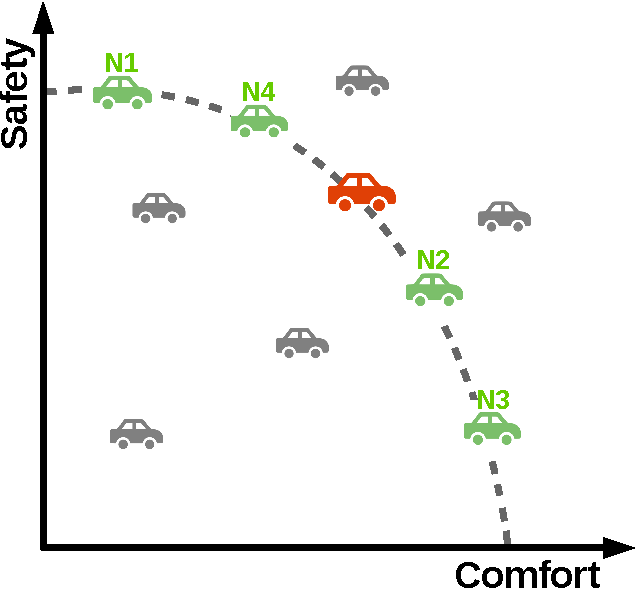
\includegraphics[width=0.35\textwidth]{figs/pareto-croped.pdf}
  \caption{{\fontsize{10}{10}\selectfont Pareto optimal decisions for the
  neighbors.}}
  \label{fig:pareto}
\end{figure}

Let's consider two general objectives, \textit{Safety} and \textit{Comfort}, for
any driver while driving between the source and the destination. Indeed, all the
drivers would like to maximize both of these objectives. However, while they
need to obey the traffic law, they need to take into account their neighbors'
driving behaviors, and respect their objectives. In the example shown in Figure
\ref{fig:pareto}, the red car's driver wants to maximize her own safety and
comfort to her aspiration level for both objectives to obtain the ``preferred''
point. We believe at least for certain redius, the red vehicle should consider
objectives of the other vehicles in that neighborhood (four vehicles shown in
green), and update their anticipated and its own state based on their behaviors.
To achieve this goal, a cognitive system should be able to make decisions with
which it is impossible to change the state of self better off without making the
state of at least one of the neighbors worse off. Therefore, the cognitive
system's decision for any given event should be a pareto optimal solution, since
the neighboring connected vehicles' objectives are important for each individual
vehicle. Here, we only used the concept of pareto optimality to discuss the type
of decisions a cognitive system of a vehicle should make. Our cognitive system
and the underlying mechanisms do not take a game theoretic approach to make
decisions.

\subsection{Cognition Systems}

Integration of cogniton into connected vehicles needs us to understand the
building blocks of cognition, how do they relate to each other, and what
functional operations they provide. We choose Newell's general theory of
cognitive control, PEACTIDM \cite{newell:unified-cognition}, to describle the
underlying abstract processes of a cognitive system. PEACTIDM is a theory of
cognitive control where cognition is decomposed into a set of eight abstract
functional operations \cite{newell:unified-cognition} all of which are
hypothesized as the building blocks of one's immediate behavior. Figure
\ref{fig:peactidm} shows the sequence of PEACTIDM's building blocks.

\textit{Perceive} is the reception of raw sensory data. For instance, connected
vehicles receive data from both their own local sensory system (e.g., GPS) and
their neighbor vehicles (e.g., an abrupt change in their velocities).
\textit{Encode} is the transformation of the sensory data into features that the
cognitive system can process. In the cognitive architectures using Bratman's BDI
paradigm \cite{bratman:intentions-plans} each sensory data will be tranformed
into a new \textit{belief}. The cognitive architecture will be able to use these
beliefs in different processes. For example, in connected vehicles there will be
a belief about the current accelaration value of the vehicle which corresponds
to the sensory data indicating this value. \textit{Attend} is the act of
shifting or maintaining the focus of attention on an event. For instance, an
alert raised because of a sudden speed reduction of multiple leading neighbor
vehicles needs to be attended immediately while the same alert does not need the
same level of attention if the leading vehicles are a few miles apart.
\textit{Comprehend} is the act of trnasforming an event into a goal or
task-spcific representation and inferring the curent status of the world. For
instance, a vehicle receiving an alert requiring an immediate reaction needs to
identify the cause of the problem even though the alert has raised and received
from another vehicle. Thus, the receiver of the alert can apply replanning if
necessary.

\begin{figure}[tbh]
  \centering
  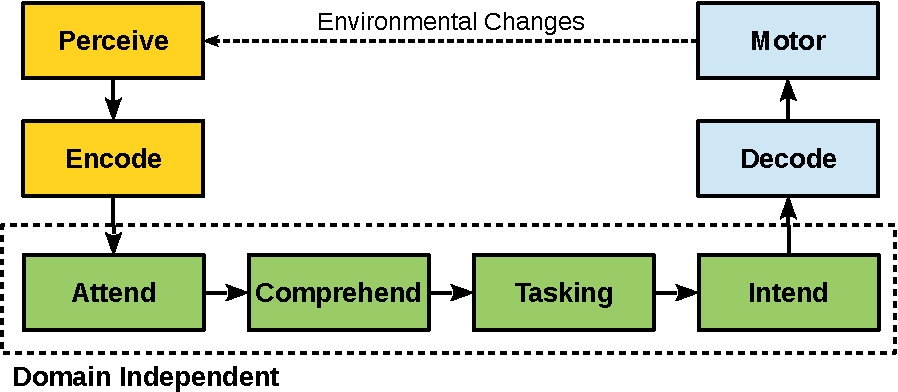
\includegraphics[width=0.485\textwidth]{figs/peactidm-croped.pdf}
  \caption{{\fontsize{10}{10}\selectfont PEACTIDM}}
  \label{fig:peactidm}
\end{figure}

\textit{Tasking} is the process of recognizing a goal based on the new state of
the world. For example, a vehicle can recognize a goal in the plan to exit the
highway with respect to the new beliefs about an accident a few miles ahead and
the current state of the highway which causes constant speed reduction.
\textit{Intend} initiates a future action based on the current goal as response
to the current event. For instance, if the current goal of the vehicle is to
leave the highway, the vehicle begins to change the lane to the right most to be
able to take the next exit. \textit{Decode} translates the response based on the
given \textit{intention} into a series of motor actions. For instance, if the
intention is changing the lane to the right, The vehicle applies a series of
actions including using the right blinker, checking the occupancy status of the
right lane, and turning the steering wheel to the right whenever it is
appropriate. \textit{Motor} executes the actions decoded based on the given
intention. For example, in case of a lane change, the blinker starts to blink
and the wheels turn to the right respective to the amount of change on the
steering wheel.

\section{{\fontsize{11.5}{9}\selectfont Affective Motivational Collaboration
Theory}}
\label{sec:amct}

\textit{Affective Motivational Collaboration Theory} is about the interpretation
and prediction of observable behaviors in a dyadic collaborative interaction.
Affective Motivational Collaboration Theory specifies the processes involved in
the progress of a collaboration and how they impact the collaboration's
underlying structure. This theory is built on the foundations of the
\textit{SharedPlans} theory of collaboration \cite{grosz:plans-discourse} and
the \textit{cognitive appraisal} theory of emotions
\cite{gratch:domain-independent}.

The theory focuses on the processes regulated by emotional states. It aims to
explain both rapid emotional reactions to events as well as slower, more
deliberative responses. The observable behaviors represent the outcome of
reactive and deliberative processes related to the interpretation of the self's
relationship to the collaborative environment. Affective Motivational
Collaboration Theory aims to explain both rapid emotional reactions to events as
well as slower, more deliberative responses. The reactive and deliberative
processes are triggered by two types of events: \textit{external} events, such
as the other's \textit{nonverbal behaviors} and \textit{primitive actions}, and
\textit{internal} events, comprising changes in the self's mental states, such
as belief formation and emotional changes.

Affective Motivational Collaboration Theory explains how emotions regulate the
underlying processes when these events occur during collaboration. This theory
elucidates the role of motives as goal-driven affect-regulated constructs with
which an agent can form new intentions to cope with internal and external
events. Therefore, a new motive can become a new intention and the self can take
a new action based on the new intention.  The focus of underlying mechanisms is
on the ones depicted as mental processes in Figure \ref{fig:cpm} along with the
mental states.

\begin{figure}[tbh]
  \centering
  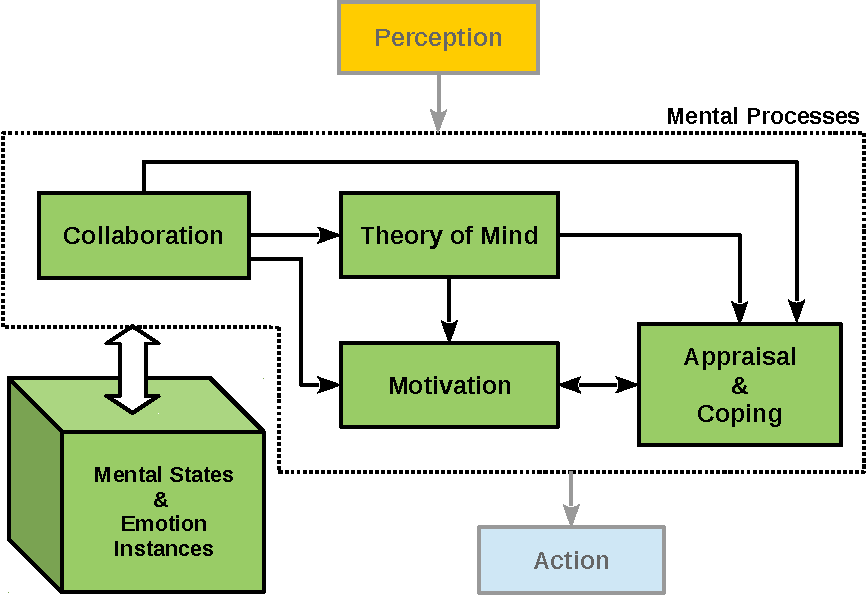
\includegraphics[width=0.485\textwidth]{figs/theory-general-croped.pdf}
  \caption{{\fontsize{10}{10}\selectfont Computational framework based on
  Affective Motivational Collaboration Theory (arrows indicate primary
  influences between mechanisms).}}
  \label{fig:cpm}
\end{figure}

The \textit{Mental States} includes ego's (vehicle's) beliefs, intentions,
motives, goals and emotion instances as well as the anticipated Mental States of
the neighbors (other vehicles). For instance, every sensory data, every
threshold value, or every inferred information about the world has a
corresponding belief in the Mental States. The \textit{Collaboration} mechanism
maintains constraints on actions, including task states and the ordering of
tasks. Although maintaining safety and comfort is a goal for each individual
vehicle, all vehicles also have a shared goal to achieve which is sharing the
road with others -- at least partially -- to get to their destinations.
Therefore, vehicles require a mechanism to maintain their full or partial shared
plan. The \textit{Collaboration} mechanism also provides processes to update and
monitor the shared plan. The \textit{Appraisal} mechanism is responsible for
evaluating changes in the ego's Mental States, the anticipated Mental States of
the neighbors, and the state of the collaboration environment. The outcome of
appraisal impacts every vehicle as an evaluative, regulatory, or motivative
process. For instance, \textit{expectedness} of an event indicates how prepared
is the ego to cope with the event, or how to maintain current state with respect
to the current changes in neighbors' location. The \textit{Coping} mechanism
provides the ego with different coping strategies associated with changes in the
ego's mental states with respect to the state of the collaboration. For
instance, does ego need to change speed with respect to the current state of
the road, or does it need to replan to get to the destination. The
\textit{Motivation} mechanism operates whenever the ego a) requires a new
motive to form a new intention with respect to current event, or b) wants to
interpret a neighbor's motive whenever the neighbor's behavior triggers an
alarm after ego appraising the situation. The \textit{Theory of Mind} mechanism
is the mechanism that infers a model of the neighbor's anticipated mental state.
The ego progressively updates this model during the collaboration. A neighbor's
model impacts ego's decision with respect to the state of the neighbor.

\section{Proposed Cognition Mechanism in Connected Vehicles}
\label{sec:cogInCv}
%

%
%
%
%%%%%%%%%%%
%
%
%
%
\section{Case Study}
\label{sec:caseStudy}
%
%
\section{Future Works}
\label{sec:futureWorks}
%
%
%
%\begin{figure}[!h]
%\centerline{\epsfig{figure =figs/PerrorSurface.eps, height=1.8 in}}
%\caption{Probability of incorrect detection by changing SNR and detection threshold. For each SNR value, there is only one minimum point since the the function is convex.}\label{PerrorSurface} 
%\end{figure}
%


\section{Conclusion}
\label{Conc}
%

\bibliographystyle{IEEEtran}
\bibliography{mshayganfar}
% \bibliography{referencesVTM}
\end{document}
